\documentclass[tikz,border=2pt]{standalone}
\usepackage{amsmath}
\usepackage{pgfplots}
\pgfplotsset{compat=1.18}

\begin{document}
% On [a,b] the global maximum is the largest of all values (here at the endpoint b), beating the
% local maximum inside; the global minimum is attained at the interior local minimum.
% f(x) = (x-1.9)^3 - 1.8(x-1.9) + 0.4 on [0.7, 3.6]: f(0.7)=0.832, local max f(1.125)=1.33,
% local & global min f(2.675)=-0.53, global max f(3.6)=2.25.
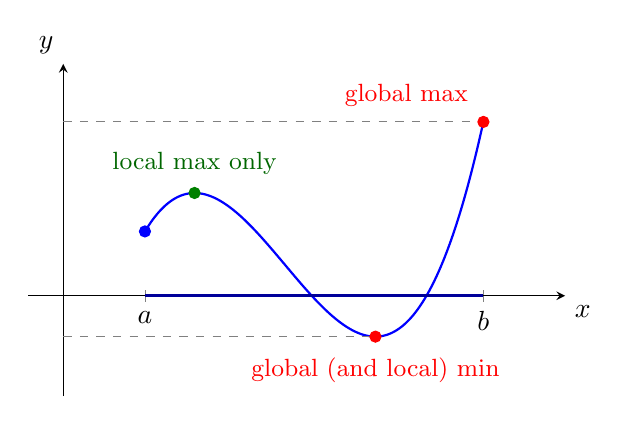
\begin{tikzpicture}
	\begin{axis}[
		axis lines=middle,
		xmin=-0.3, xmax=4.3,
		ymin=-1.3, ymax=3.0,
		xtick={0.7,3.6}, xticklabels={$a$,$b$},
		ytick=\empty,
		xlabel={$x$}, ylabel={$y$},
		xlabel style={below right}, ylabel style={above left},
		samples=200, smooth, clip=false,
		width=8.4cm, height=5.8cm
		]
		\addplot[thick, blue, domain=0.7:3.6] {(x-1.9)^3-1.8*(x-1.9)+0.4};
		\addplot[only marks, mark=*, blue] coordinates {(0.7,0.832)};
		\addplot[only marks, mark=*, green!50!black] coordinates {(1.125,1.33)};
		\addplot[only marks, mark=*, red] coordinates {(2.675,-0.53) (3.6,2.25)};
		\node[green!40!black, anchor=south, font=\small] at (axis cs:1.125,1.45) {local max only};
		\node[red, anchor=north, font=\small] at (axis cs:2.675,-0.68) {global (and local) min};
		\node[red, anchor=south east, font=\small] at (axis cs:3.55,2.33) {global max};
		\draw[dashed, gray] (axis cs:0,2.25) -- (axis cs:3.6,2.25);
		\draw[dashed, gray] (axis cs:0,-0.53) -- (axis cs:2.675,-0.53);
		\draw[blue!60!black, very thick] (axis cs:0.7,0) -- (axis cs:3.6,0);
	\end{axis}
\end{tikzpicture}
\end{document}
